\subsection{Strategi Persiapan Dataset}
\label{subsec:strategi-persiapan-dataset}

Persiapan \dataset{} merupakan tahapan kritis dalam pengembangan sistem ekstraksi data pembayaran. Strategi persiapan \dataset{} dirancang untuk memastikan kualitas dan representativitas data yang akan digunakan untuk melatih model \donut{} yang telah disesuaikan dengan domain pembayaran Indonesia.

\datasetfl{} yang disiapkan mencakup gambar bukti pembayaran dari berbagai jenis aplikasi pembayaran digital dan struk kertas. \datasetfl{} struk kertas yang digunakan untuk melatih model \donut{} adalah \dataset{} CORD-V2\footnote{\href{https://huggingface.co/datasets/naver-clova-ix/cord-v2}{https://huggingface.co/datasets/naver-clova-ix/cord-v2}} (\emph{Consolidated Receipt Dataset for Post-OCR Parsing}). \datasetfl{} ini dibagi menjadi 800 data latih, 100 data validasi, dan 100 data uji. \datasetfl{} ini digunakan untuk melatih model \donut{} agar dapat mengenali dan mengekstrak informasi dari struk pembayaran. \datasetfl{} ini memiliki keterbatasan, yaitu memiliki bagian yang di-\emph{blur}. Keterbatasan ini membuat \donut{} mengalami kesulitan untuk memprediksi struk pembayaran yang penuh.
\begin{figure}[htbp]
    \centering
    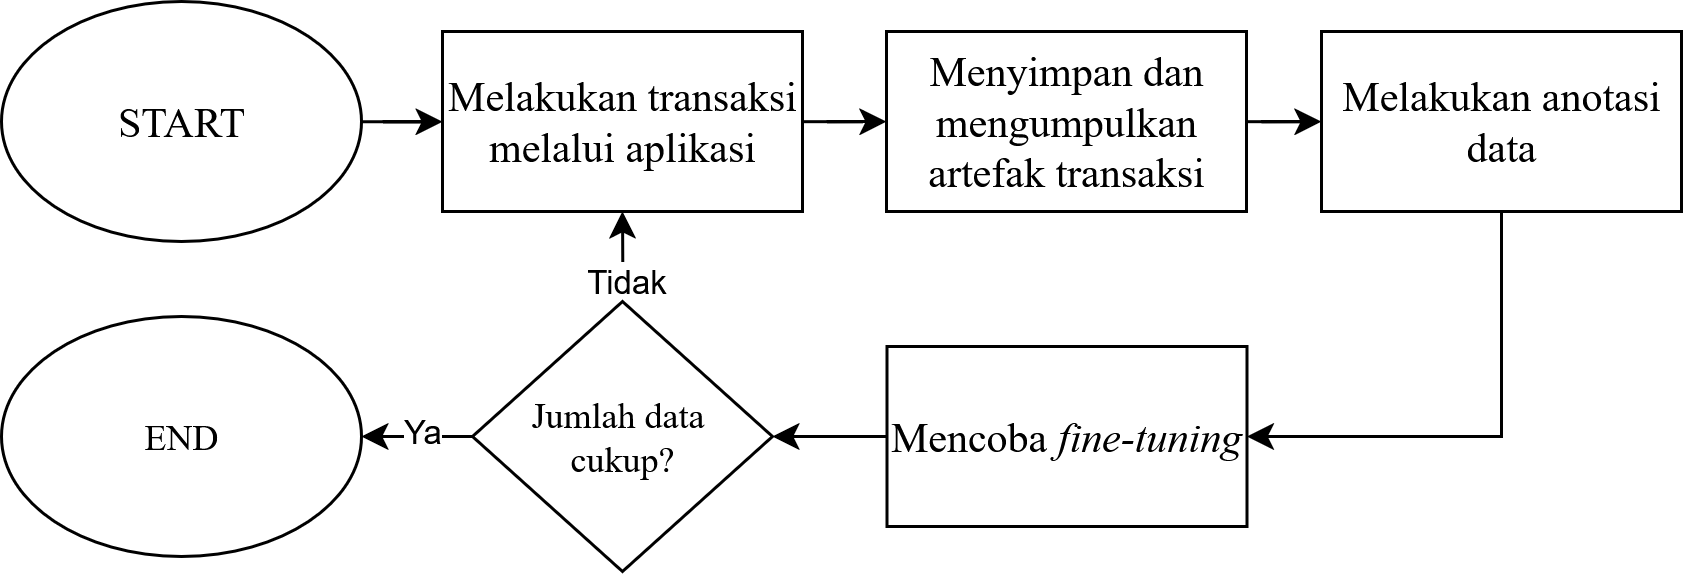
\includegraphics[width=1\textwidth]{images/dataset-preparation-flow.png}
    \caption{Alur kerja persiapan \dataset{} QRIS dan transfer bank}
    \label{fig:dataset-preparation-flow}
\end{figure}

\datasetfl{} yang digunakan untuk melatih model \donut{} adalah \dataset{} QRIS dan transfer yang berisi gambar bukti pembayaran dari berbagai aplikasi pembayaran digital seperti SeaBank, Neobank, BCA, dan \gopay{} yang perlu dipersiapkan secara sistematis. \autoref{fig:dataset-preparation-flow} menunjukkan alur kerja sistematis dalam persiapan \dataset. Proses dimulai dengan melakukan transaksi melalui aplikasi pembayaran dan mengumpukan gambar bukti pembayaran dari berbagai sumber, yaitu aplikasi pembayaran digital (SeaBank, Neobank, BCA, dan \gopay). Total \dataset{} yang dikumpulkan adalah 350 gambar bukti pembayaran QRIS dan transfer dengan format dan jenis dokumen yang bervariasi.

Gambar bukti pembayaran yang telah dikumpulkan kemudian dianotasi secara manual. Proses anotasi dilakukan secara manual untuk menandai informasi penting pada gambar dan memastikan bahwa data yang dianotasikan sesuai dengan yang tertera pada gambar bukti pembyaran. Atribut yang dianotasikan dari gambar bukti pembayaran adalah sebagai berikut:
\begin{enumerate}
    \item \iden{}: Kode transaksi yang unik untuk setiap bukti pembayaran.
    \item \total{}: Jumlah pembayaran yang tercantum pada bukti pembayaran.
    \item \ttime{}: Waktu transaksi yang tercatat pada bukti pembayaran.
    \item \target{}: Nama penerima atau tujuan pembayaran.
    \item \app{}: Aplikasi yang digunakan untuk melakukan transaksi.
    \item \type{}: Jenis dokumen berupa QRIS atau transfer.
\end{enumerate}

Proses anotasi ini dilakukan dengan cermat untuk memastikan bahwa setiap informasi yang diperlukan dapat diekstraksi dengan akurat oleh model \donut{}. Hasil anotasi kemudian disimpan dalam format JSON dan kemudian dikonversi menjadi format yang sesuai untuk pelatihan model \donut{}, yaitu format JSONL. 

\datasetfl{} yang telah dianotasi ini kemudian dibagi menjadi tiga subset, yaitu data latih, data validasi, dan data uji. Pembagian dilakukan dengan mempertimbangkan distribusi jenis dan variasi jenis dokumen untuk memastikan bahwa setiap subset mencakup representasi yang baik dari keseluruhan \dataset. Data latih digunakan untuk \emph{fine-tuning} model, data validasi untuk proses pelatihan, sedangkan data uji digunakan untuk evaluasi akhir kinerja model. 

\emph{Fine-tuning} model kemudian dilakukan untuk memastikan data yang cukup dan tidak mengandung bias yang dapat menyebabkan \emph{overfitting} pada model. Proses pengumpulan data kemudian dihentikan setelah jumlah data dinilai cukup untuk melatih model \donut{} dengan baik.